\documentclass{beamer}
\usepackage{graphicx}
\graphicspath{ {./images/} }
\usepackage[
backend=bibtex,
style=alphabetic,
citestyle=authoryear
]{biblatex}
\addbibresource{iforest.bib}

\mode<presentation>
{
  \usetheme{default}      % or try Darmstadt, Madrid, Warsaw, ...
  \usecolortheme{seahorse} % or try albatross, beaver, crane, ...
  \usefonttheme{default}  % or try serif, structurebold, ...
  \setbeamertemplate{navigation symbols}{}
  \setbeamertemplate{caption}[numbered]
}

\title{Isolation Forest and Its Extensions}
\author{Boston Lee}
\institute{Colorado State University}
\date{}

\begin{document}


\begin{frame}
  \titlepage
\end{frame}

\section{Anomaly Detection Background}

\begin{frame}{What is an anomaly?}
    \begin{itemize}
        \item We have an intuitive defintion of an anomaly, but how do we
            formalize it?
        \item A few rudimentary ideas:
            \begin{enumerate}
                \item Points generated from a different distribution than
                    ``normal'' points
                \item Points that are unusual in a given context
                \item Points that are further away from their neighbors than
                    other points
                \item Points that are few and different compared to normal points
            \end{enumerate}
    \end{itemize}
\end{frame}

\begin{frame}{Complications of Anomaly Detection}
    \begin{itemize}
        \item Unbalanced categories require adaptation of machine learning
            methods
        \item Many methods assign an ``anomaly score'' to circumvent this
            problem.
        \item Distance-based anomaly-detection can be computationally expensive
        \item Many standard methods fall prey to the curse of dimensionality
    \end{itemize}
\end{frame}

\section{Isolation Forest}

\begin{frame}{Overview}
    \begin{itemize}
        \item Isolation Forest (iForest) is a tree ensemble method, taking
            inspiration from decision trees.
        \item Isolation Forest does not make any distributional assumptions
            about anomalies. It uses the heuristic that anomalies are ``few and
            different'': In other words, anomalies are \textit{easy to isolate}
            \cite{liu2009}.
    \end{itemize}
\end{frame}

\begin{frame}{Formalizing iForest: Isolation Trees}
    \begin{itemize}
        \item An isolation forest is built out of isolation trees.
        \item Isolation trees are formed by random splits on random predictors
        \item We split the data randomly because anomalies should be easier to
            separate from the data.
    \end{itemize}
\end{frame}

\begin{frame}{Formalizing iForest, cont.}
    \begin{itemize}
        \item Within an isolation tree, a point's anomaly status is measured by
            how deep in the tree it is: The less splits it takes to isolate a
            point, the more anomalous it is.
    \end{itemize}
\end{frame}

\begin{frame}{Visualizing Structure}
    \begin{center}
        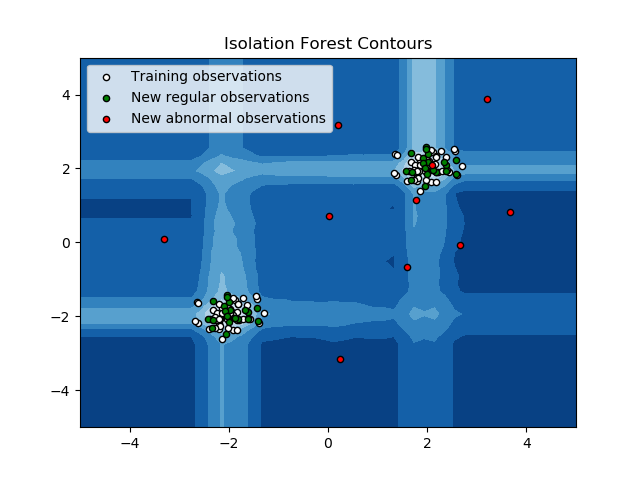
\includegraphics[width=\textwidth]{example_visualization}
    \end{center}
\end{frame}

\begin{frame}

    Once we have a collection of isolation trees, we can aggregate the path length
    for each point across the trees, removing variability.  Formally, for a set of
    $n$ observations, the anomaly score can be defined as:

    \begin{equation*}
        s(x,n) = 2^{- \frac{E(h(x))}{c(n)}}
    \end{equation*}

    where $E(h(x))$ is the average path length across a collection of
    \textit{iTree}s, and $c(n)$ is the average path length of an unsuccessful
    binary search in a dataset of size $n$ \cite{liu2009}.

\end{frame}

\begin{frame}
    \printbibliography
\end{frame}

\end{document}
